% =====================================================================
%  第 1 章 希尔伯特空间形式 —— ch01b（§1.6–§1.8）
%  页段：PDF 31–48（原书 p.30–47）
% =====================================================================

% [本块起于原书 p.30，§1.5.4 定态的收尾一段。上接 ch01a 末句“……本征值 $E$ 自然被理解为该态 $\psi$ 的能量。”]

% [原文 p.30]
方程 $(*)$ 称为\emph{定态薛定谔方程}（time-independent Schrödinger equation）。由于 $\hat H$ 自伴，$E$ 必为实数。

形如
\[
\Psi(\mathbf{x},t)=\ee^{-\ii Et/\hbar}\psi(\mathbf{x})
\qquad\text{且}\qquad
\hat H\psi=E\psi
\]
的解也称为\emph{定态}（stationary states）。概率密度
\[
\abs{\Psi(\mathbf{x},t)}^2=\abs{\psi(\mathbf{x})}^2
\]
不依赖时间 $t$。这些态在任意时刻都是哈密顿量 $\hat H$ 的本征态
\[
\hat H\Psi(\mathbf{x},t)=E\Psi(\mathbf{x},t).
\]
特别地，态 $\Psi$ 中 $\hat H$ 的期望为
\[
\expv{\hat H}_{\Psi}=E,
\]
而 $\hat H$ 在态 $\Psi$ 中的不确定度为零
\[
\Delta_{\Psi}\hat H=0.
\]

一旦求出全部能量为 $E_{\alpha}$ 的定态 $\psi_{\alpha}$，薛定谔方程的通解即可写成叠加
\[
\sum_{\alpha}c_{\alpha}\ee^{-\ii E_{\alpha}t/\hbar}\psi_{\alpha}(\mathbf{x}).
\]
因此，先把定态弄清楚是根本的，也就是研究定态薛定谔方程。一般说来，$\hat H$ 可以既有离散谱又有连续谱。对连续谱，上面的求和 $\sum_{\alpha}$ 要换成适当的积分。离散谱与连续谱都有特定的物理含义。后文将用若干谱型不同的例子加以说明。谱的精确数学描述见 §4.2。

% [§1.5 的本节重点：本节跨 ch01a/ch01b 两块，takeaway 放在本节真正结束处]
\takeaway{本节把抽象的希尔伯特空间向量落实为 $\R^n$ 上的波函数：位置算子是乘法、动量算子是 $-\ii\hbar\nabla$，正则对易关系与海森堡不等式随之成立；哈密顿算子是微分算子，这使总概率的守恒可以写成局域的连续性方程，并由概率流描述；最后把时间分离出去，得到定态与不含时薛定谔方程。}

\section{自由粒子：连续谱的例子}

\subsection{波包}

考虑势 $V=0$ 的自由量子粒子。哈密顿量为
\[
\hat H=-\frac{\hbar^2}{2m}\nabla^2.
\]
自由薛定谔方程
\[
\ii\hbar\frac{\pa}{\pa t}\psi(\mathbf{x},t)=-\frac{\hbar^2}{2m}\nabla^2\psi(\mathbf{x},t)
\]

% [原文 p.31]
有平面波解
\[
\psi_{\mathbf{k}}(\mathbf{x},t)=\ee^{\ii(\mathbf{k}\cdot\mathbf{x}-\omega(\mathbf{k})t)}.
\]
这里波矢 $\mathbf{k}$ 与角频率 $\omega$ 由动量 $\mathbf{p}$ 和能量 $E$ 决定：
\[
\mathbf{p}=\hbar\mathbf{k},\qquad E=\hbar\omega.
\]
它们称为\emph{德布罗意关系}（de Broglie relations），对一般物质波都成立。

用 $\hat H=-\frac{\hbar^2}{2m}\nabla^2$，得到 $E=\frac{\mathbf{p}^2}{2m}$，即
\[
\omega(\mathbf{k})=\frac{\hbar\mathbf{k}^2}{2m}.
\]
这给出此情形下的色散关系。

然而，平面波解 $\Psi_{\mathbf{k}}$ 不可归一化：
\[
\abs{\Psi_{\mathbf{k}}}^2=1
\qquad\text{对任意}\ \mathbf{x}\ \text{与}\ t.
\]
$\abs{\Psi_{\mathbf{k}}}^2$ 在全空间的积分是无穷大。所以 $\Psi_{\mathbf{k}}$ 不给物理态。

尽管如此，一般解可由平面波叠加成波包：
\[
\Psi(\mathbf{x},t)=\frac{1}{(2\pi\hbar)^{n/2}}\int\rd^n\mathbf{p}\ \hat\psi_0(\mathbf{p})\,\ee^{\ii(\mathbf{p}\cdot\mathbf{x}-E(\mathbf{p})t)/\hbar}.
\]
显然，记 $\psi_0(\mathbf{x})$ 为 $t=0$ 时的波函数
\[
\psi_0(\mathbf{x})=\Psi(\mathbf{x},0).
\]
则 $\hat\psi_0(\mathbf{p})$ 是 $\psi_0(\mathbf{x})$ 到动量空间的傅里叶变换。这就由 $t=0$ 时的给定量初值给出了波函数的显式解。

\begin{example}{1.6.1}
  （\textbf{高斯波包}）考虑一维情形 $n=1$。取 $t=0$ 时的初始波函数为
  \[
  \psi_0(x)=\ee^{\ii p_0x/\hbar}\frac{\ee^{-x^2/4\delta^2\hbar}}{(2\pi\delta^2\hbar)^{1/4}},
  \qquad \delta>0.
  \]
  系数之选取使归一化条件成立
  \[
  \int_{\R}\rd x\,\abs{\psi_0(x)}^2
  =\frac{1}{\sqrt{2\pi\hbar}\,\delta}\int_{\R}\rd x\,\ee^{-x^2/2\delta^2\hbar}=1.
  \]
  $\abs{\psi_0(x)}^2=\dfrac{\ee^{-x^2/2\delta^2\hbar}}{\sqrt{2\pi\hbar}\,\delta}$ 的大小是高斯型的。

  \begin{center}
    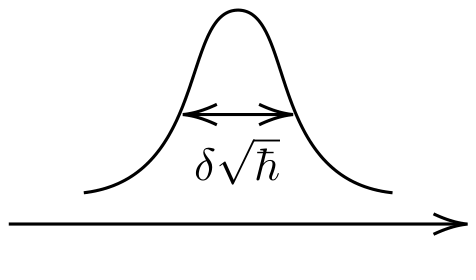
\includegraphics[width=0.52\textwidth]{figures/fig_p32_a.png}
  \end{center}
  % [图：原书 p.31，原图无题注]

  % [原文 p.32]
  参数 $\delta$ 联系着 $\hat x$ 的不确定度
  \[
  \Delta_{\psi_0}\hat x
  =\left(\int_{\R}\rd x\,x^2\abs{\psi_0(x)}^2\right)^{1/2}
  =\delta\sqrt{\hbar}.
  \]
  $\psi_0(x)$ 的傅里叶变换是
  \[
  \begin{aligned}
  \hat\psi_0(p)&=\int_{\R}\rd x\,\ee^{-\ii px/\hbar}\psi_0(x)\\
  &=\int_{\R}\rd x\,\ee^{-\ii(p-p_0)x/\hbar}
  \frac{\ee^{-x^2/4\delta^2\hbar}}{(2\pi\hbar\delta^2)^{1/4}}\\
  &=\frac{\ee^{-(p-p_0)^2\delta^2/\hbar}}
  {\left((2\pi\hbar)^{-1}(2\delta)^{-2}\right)^{1/4}}.
  \end{aligned}
  \]
  借助 $\hat\psi_0$ 可算出动量算子 $\hat p$ 的不确定度
  \[
  \Delta_{\psi_0}\hat p=\frac{\sqrt{\hbar}}{2\delta}.
  \]
  于是得到海森堡不确定性
  \[
  \Delta_{\psi_0}\hat x\cdot\Delta_{\psi_0}\hat p=\frac{\hbar}{2}.
  \]

  任意时刻 $t$ 的波函数由此解出
  \[
  \begin{aligned}
  \Psi(x,t)&=\frac{1}{2\pi\hbar}\int_{\R}\rd p\,\hat\psi_0(p)\,\ee^{\ii(px-p^2t/2m)/\hbar}\\
  &=\frac{1}{2\pi\hbar}\int_{\R}\rd p\,
  \frac{\ee^{-(p-p_0)^2\delta^2/\hbar}}
  {\left((2\pi\hbar)^{-1}(2\delta)^{-2}\right)^{1/4}}
  \ee^{\ii(px-p^2t/2m)/\hbar}\\
  &=\frac{1}{\left(\sqrt{2\pi\hbar}\left(\delta+\dfrac{\ii t}{2m\delta}\right)\right)^{1/2}}
  \ee^{\frac{\ii p_0}{\hbar}\left(x-\frac{p_0t}{2m}\right)}
  \exp\left(-\frac{\left(x-\frac{p_0t}{m}\right)^2}
  {4\left(\delta^2+\dfrac{\ii t}{2m}\right)\hbar}\right).
  \end{aligned}
  \]
\end{example}

\subsection{群速度}

我们想弄清一个局域化的波包如何在空间中移动。先看如下一般的一维波包：
\[
\Psi(x,t)=\frac{1}{\sqrt{2\pi}}\int\rd k\,\hat\phi_0(k)\,\ee^{\ii(kx-\omega(k)t)}.
\]
这里做傅里叶变换用的是波矢 $k$，而不用动量 $p=\hbar k$。$\omega(k)$ 是 $k$ 的函数，描述色散关系。

设 $\hat\phi_0(k)$ 集中在 $k=k_0$ 附近，即只有 $k\sim k_0$ 时才有贡献。

\begin{center}
  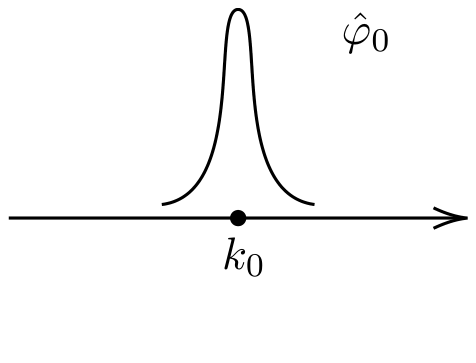
\includegraphics[width=0.52\textwidth]{figures/fig_p33_a.png}
\end{center}
% [图：原书 p.32，原图无题注]

% [原文 p.33]
我们要问：$x$ 与 $t$ 取什么值时，波包 $\Psi(x,t)$ 的模最大。当 $k\sim k_0$ 时，可作近似
\[
\omega(k)\simeq\omega(k_0)+\omega'(k_0)(k-k_0).
\]
把它代入波包，得
\[
\begin{aligned}
\Psi(x,t)&=\frac{1}{\sqrt{2\pi}}\int\rd k\,\hat\phi_0(k)\,\ee^{\ii(kx-\omega(k)t)}\\
&\simeq\frac{1}{\sqrt{2\pi}}\ee^{-\ii\omega(k_0)t+\ii k_0\omega'(k_0)t}
\int\rd k\,\hat\phi_0(k)\,\ee^{\ii k(x-\omega'(k_0)t)}\\
&=\ee^{-\ii\omega(k_0)t+\ii k_0\omega'(k_0)t}\Psi(x-\omega'(k_0)t,0).
\end{aligned}
\]
设初始波函数 $\Psi(x,0)$ 的模的峰值在 $x=x_0$。上面的计算表明，时刻 $t$ 波包 $\Psi(x,t)$ 的模的峰值近似出现在
\[
x=\omega'(k_0)t+x_0.
\]
换言之，波包的峰值以速度 $\omega'(k_0)$ 移动。这称为\emph{群速度}（group velocity）：
\[
\text{群速度}=\left.\frac{\rd\omega}{\rd k}\right|_{k=k_0}.
\]
它描述波包传播的近似速率。

与之相对，还有\emph{相速度}（phase velocity）的概念，定义为
\[
\text{相速度}=\left.\frac{\omega}{k}\right|_{k=k_0}.
\]
它描述纯平面波 $\ee^{\ii(k_0x-\omega(k_0)t)}$ 传播的速率。

对线性色散关系
\[
\omega(k)=\alpha k
\qquad\text{其中}\quad \alpha=\text{常数},
\]
群速度与相速度重合，都等于 $\alpha$。真空中的电磁波就是这样的例子。

一般情形下群速度与相速度不同。以一维自由量子粒子为例。德布罗意关系
\[
p=\hbar k,\qquad E=\hbar\omega
\]
与 $E=p^2/2m$ 一起给出色散关系
\[
\omega(k)=\frac{\hbar k^2}{2m}.
\]
对动量集中在 $p_0=\hbar k_0$ 的波包，群速度为
\[
\left.\frac{\rd\omega}{\rd k}\right|_{k=k_0}
=\frac{\hbar k_0}{m}=\frac{p_0}{m}.
\]

% [原文 p.34]
这正是动量为 $p_0$、质量为 $m$ 的自由粒子应有的速度。作为对比，相速度为
\[
\left.\frac{\omega}{k}\right|_{k=k_0}
=\frac{\hbar k_0}{2m}=\frac{p_0}{2m}.
\]
在高斯波包例 1.6.1 中，
\[
\Psi(x,t)=\frac{1}{\left(\sqrt{2\pi\hbar}\left(\delta+\dfrac{\ii t}{2m\delta}\right)\right)^{1/2}}
\ee^{\frac{\ii p_0}{\hbar}\left(x-\frac{p_0t}{2m}\right)}
\exp\left(-\frac{\left(x-\frac{p_0t}{m}\right)^2}
{4\left(\delta^2+\dfrac{\ii t}{2m}\right)\hbar}\right).
\]
$\hbar$ 很小时，动量模式 $\hat\psi_0(p)$ 集中在 $p_0$ 附近。于是清楚看到，$\Psi(x,t)$ 的峰值以群速度 $p_0/m$ 行进。

\takeaway{本节用平面波叠加造出波包，给出自由粒子的连续谱。波包不是单个平面波，其峰值按群速度 $\rd\omega/\rd k$ 移动，而平面波本身按相速度 $\omega/k$ 移动；对自由粒子，两者分别等于 $p_0/m$ 与 $p_0/2m$。}

\section{谐振子：离散谱的例子}

本节研究谐振子这一可精确求解的例子。它是量子物理中最重要的模型之一。

为简单起见，我们只看一维情形。经典哈密顿量为
\[
\mathcal H=\frac{p^2}{2m}+\frac12 kx^2,
\]
其中 $m$ 是粒子质量，$k>0$ 是常数。势 $V=\frac12 kx^2$ 关于 $x$ 是二次的，且不依赖时间。

经典地，粒子的运动服从哈密顿方程
\[
\begin{cases}
\dot x=\dfrac{\pa\mathcal H}{\pa p}=\dfrac{p}{m},\\[3mm]
\dot p=-\dfrac{\pa\mathcal H}{\pa x}=-kx.
\end{cases}
\]
关于 $x$ 的运动方程是
\[
m\ddot x=-kx.
\]
作用在粒子上的力由胡克定律给出，$F=-kx$。

\begin{center}
  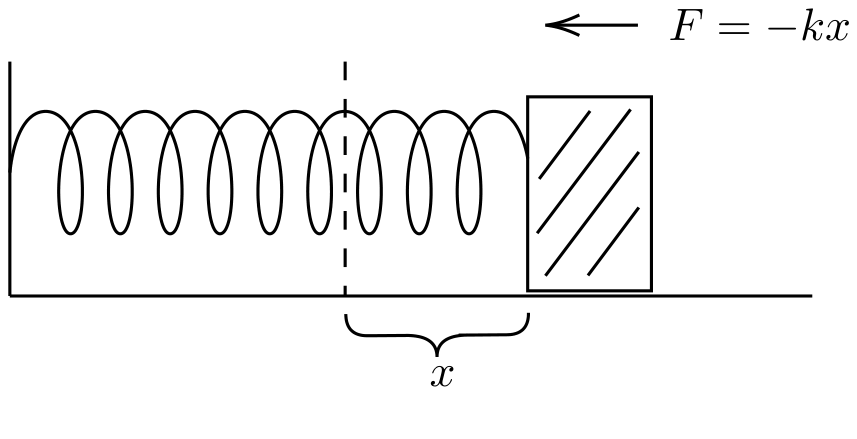
\includegraphics[width=0.60\textwidth]{figures/fig_p35_a.png}
\end{center}
% [图：原书 p.34，原图无题注]

运动方程的解为
\[
x(t)=A\cos\omega t+B\sin\omega t,
\]
其中 $A,B$ 是常数，而
\[
\omega=\sqrt{\frac{k}{m}}
\]

% [原文 p.35]
是振动的角频率。

量子力学中，哈密顿算子是
\[
\hat H=-\frac{\hbar^2}{2m}\frac{\rd^2}{\rd x^2}+\frac12 kx^2.
\]
只需求解关于定态 $\psi(x)$ 的定态薛定谔方程
\[
\hat H\psi(x)=E\psi(x).
\]
相应的波函数随即由 $\psi(x,t)=\psi(x)\ee^{-\ii Et/\hbar}$ 给出。

\subsection{阶梯算子}

注意，谐振子的定态薛定谔方程可以用简单的代数方法精确求解。记
\[
\hat H=\frac{\hat p^2}{2m}+\frac{k}{2}\hat x^2
=\frac{\hat p^2}{2m}+\frac{m\omega^2}{2}\hat x^2,
\]
其中 $\hat x$ 是位置算子，$\hat p=-\ii\hbar\frac{\rd}{\rd x}$ 是动量算子。$\hat x$ 与 $\hat p$ 满足正则对易关系
\[
[\hat x,\hat p]=\ii\hbar.
\]
我们可以把哈密顿算子改写为
\[
\begin{aligned}
\hat H&=\frac{1}{2m}\left(\hat p^2+m^2\omega^2\hat x^2\right)\\
&=\frac{1}{2m}\left[(m\omega\hat x-\ii\hat p)(m\omega\hat x+\ii\hat p)-\ii m\omega(\hat x\hat p-\hat p\hat x)\right]\\
&=\frac{1}{2m}(m\omega\hat x-\ii\hat p)(m\omega\hat x+\ii\hat p)+\frac12\hbar\omega\\
&=\hbar\omega\left[\frac{1}{2m\hbar\omega}(m\omega\hat x-\ii\hat p)(m\omega\hat x+\ii\hat p)+\frac12\right]\\
&=\hbar\omega\left(a^\dagger a+\frac12\right),
\end{aligned}
\]
其中引入了两个算子
\[
a^\dagger=\frac{1}{\sqrt{2m\hbar\omega}}(m\omega\hat x-\ii\hat p),
\qquad
a=\frac{1}{\sqrt{2m\hbar\omega}}(m\omega\hat x+\ii\hat p).
\]
它们称为\emph{阶梯算子}（ladder operators）。名称的来历很快会清楚。正如符号所暗示的，$a^\dagger$ 与 $a$ 互为伴随。

首先观察到，阶梯算子满足对易关系
\[
[a,a^\dagger]=1.
\]
由此得到如下对易关系
\[
[\hat H,a^\dagger]=\hbar\omega a^\dagger,
\qquad
[\hat H,a]=-\hbar\omega a.
\]
关键在于下面的陈述。

% [原文 p.36]
\begin{proposition}{1.7.1}
  若 $\psi$ 满足能量为 $E$ 的定态薛定谔方程，则 $a^\dagger\psi$（或 $a\psi$）满足能量为 $E+\hbar\omega$（或 $E-\hbar\omega$）的定态薛定谔方程。
\end{proposition}

\begin{proof}
  设 $\psi$ 满足 $\hat H\psi=E\psi$。则
  \[
  \begin{aligned}
  \hat H\left(a^\dagger\psi\right)
  &=[\hat H,a^\dagger]\psi+a^\dagger\hat H\psi\\
  &=\hbar\omega a^\dagger\psi+Ea^\dagger\psi\\
  &=(E+\hbar\omega)a^\dagger\psi.
  \end{aligned}
  \]
  $a\psi$ 的计算类似。
\end{proof}

因此，阶梯算子 $a^\dagger,a$ 让我们能在能量上爬上爬下。我们也称 $a^\dagger$ 为\emph{升算子}（raising operator），$a$ 为\emph{降算子}（lowering operator）。

\subsection{基态}

第二个关键陈述如下。

\begin{proposition}{1.7.2}
  定态的能量 $E$ 非负。
\end{proposition}

\begin{proof}
  对能量为 $E$ 的归一定态 $\psi$，
  \[
  \begin{aligned}
  E&=\langle\psi|\hat H|\psi\rangle
  =\int_{\R}\rd x\,\overline{\psi(x)}
  \left(-\frac{\hbar^2}{2m}\frac{\rd^2}{\rd x^2}+\frac12 kx^2\right)\psi(x)\\
  &=\int_{\R}\rd x\left(
  \frac{\hbar^2}{2m}\left|\frac{\rd}{\rd x}\psi(x)\right|^2
  +\frac12 kx^2\abs{\psi(x)}^2\right)\ge 0.
  \end{aligned}
  \]
  这里我们稍稍作了弊：未加证明地假设 $\psi$ 可微，且在空间无穷远处有适当的衰减条件。这一点留给更细心的读者。
\end{proof}

现给定能量为 $E$ 的定态 $\psi$，可用降算子 $a$ 把能量降下去。由于非零态的能量非负，当 $m$ 充分大时 $a^m\psi=0$。

设 $E_0\ge 0$ 是最小的能量。能量最低的态称为\emph{基态}（ground states）。取 $\psi_0$ 为一个能量为 $E_0$ 的基态。我们很快就会看到，此情形下基态（相差一个归一化）唯一。作为基态，$\psi_0$ 必满足
\[
a\psi_0=0,
\]
也就是微分方程
\[
\left(\hbar\frac{\rd}{\rd x}+m\omega x\right)\psi_0(x)=0.
\]
相差一个归一化，解唯一，由
\[
\psi_0(x)=\left(\frac{m\omega}{\pi\hbar}\right)^{1/4}\ee^{-\frac{m\omega}{2\hbar}x^2}
\]
给出。系数之选取使
\[
\int_{\R}\rd x\,\abs{\psi_0(x)}^2=1.
\]

% [原文 p.37]
相应的能量为
\[
\hat H\psi_0=\hbar\omega\left(a^\dagger a+\frac12\right)\psi_0
=\frac12\hbar\omega\psi_0
\quad\Longrightarrow\quad
E_0=\frac12\hbar\omega.
\]
注意，经典力学中谐振子可能的最小能量为零（例如静止在 $x=0$ 处的粒子）。量子力学中最小能量却是 $E_0=\frac12\hbar\omega$！这一基态能量的抬升是纯粹的量子效应。

\subsection{激发态}

从基态出发，只需作用升算子就得到更高能量的态：
\[
\psi_n(x)=A_n(a^\dagger)^n\psi_0(x)
\qquad\text{其中}\qquad
E_n=\left(n+\frac12\right)\hbar\omega,
\]
$A_n$ 是归一化常数。为算出 $A_n$，利用 $a^\dagger$ 与 $a$ 互为伴随这一事实。于是
\[
\braket{\psi_n}{\psi_n}
=\abs{A_n}^2\left\langle(a^\dagger)^n\psi_0\Big|(a^\dagger)^n\psi_0\right\rangle
=\abs{A_n}^2\langle\psi_0|a^n(a^\dagger)^n|\psi_0\rangle.
\]
利用 $a\psi_0=0$ 与 $[a,a^\dagger]=1$，可得
\[
a^n(a^\dagger)^n|\psi_0\rangle
=n\,a^{n-1}(a^\dagger)^{n-1}|\psi_0\rangle
=\cdots=n!|\psi_0\rangle.
\]
于是
\[
\braket{\psi_n}{\psi_n}=\abs{A_n}^2 n!\braket{\psi_0}{\psi_0}.
\]
归一化条件 $\braket{\psi_n}{\psi_n}=1$ 给出 $A_n=\frac{1}{\sqrt{n!}}$。所以
\[
\psi_n=\frac{1}{\sqrt{n!}}(a^\dagger)^n\psi_0.
\]
最后我们说明 $\psi_n$ 就是全部定态。

\begin{proposition}{1.7.3}
  设 $\psi$ 是能量为 $E$ 的定态。则 $\psi$ 必为某个 $n$ 的 $\psi_n$ 的形状（相差一个归一化因子），且 $E=\left(n+\frac12\right)\hbar\omega$。
\end{proposition}

\begin{proof}
  由于能量有下界，存在 $n\ge 0$ 使
  \[
  a^n\psi\ne 0,\qquad a^{n+1}\psi=0.
  \]
  于是 $a(a^n\psi)=0$。由基态的唯一性，必有
  \[
  a^n\psi=\alpha\psi_0
  \qquad\text{对某个 }\alpha\ne 0.
  \]
  比较两边，立得
  \[
  E-n\hbar\omega=E_0
  \quad\Longrightarrow\quad
  E=E_n=\left(n+\frac12\right)\hbar\omega.
  \]

  % [原文 p.38]
  设 $\psi$ 与 $\psi_n$ 线性无关。作格拉姆–施密特正交化，可设
  \[
  \braket{\psi_n}{\psi}=0.
  \]
  另一方面，利用 $a,a^\dagger$ 互为伴随这一事实，
  \[
  \braket{\psi_n}{\psi}
  \propto\left\langle(a^\dagger)^n\psi_0\Big|\psi\right\rangle
  =\langle\psi_0|a^n\psi\rangle
  =\alpha\braket{\psi_0}{\psi_0}=\alpha\ne 0.
  \]
  矛盾。故相差一个归一化，$\psi$ 与 $\psi_n$ 相同。
\end{proof}

这样我们就找到了全部定态。$n>0$ 的态 $\psi_n$ 称为\emph{激发态}（excited states），它们由基态 $\psi_0$ 作用 $a^\dagger$ 产生。注意，与经典图像不同，量子情形下能量是离散的。能量被量子化了！而且，这些态 $\{\psi_n\}_{n\ge 0}$ 构成希尔伯特空间 $L^2(\R)$ 的正交归一基（见 §4.5.2）。

基态由高斯函数显式给出：
\[
\psi_0(x)=\left(\frac{m\omega}{\pi\hbar}\right)^{1/4}\ee^{-\frac{m\omega}{2\hbar}x^2}.
\]
激发态 $\psi_n$ 可用厄米多项式显式表达。

为方便起见，重新定义变量
\[
y=\sqrt{\frac{m\omega}{\hbar}}\,x.
\]
则基态为
\[
\psi_0(x)=c_0\ee^{-y^2/2},
\qquad
c_0:=\left(\frac{m\omega}{\pi\hbar}\right)^{1/4}.
\]
阶梯算子为
\[
\begin{cases}
a^\dagger=\dfrac{1}{\sqrt{2m\hbar\omega}}\left(m\omega x-\hbar\dfrac{\rd}{\rd x}\right)
=\dfrac{1}{\sqrt2}\left(y-\dfrac{\rd}{\rd y}\right),\\[4mm]
a=\dfrac{1}{\sqrt{2m\hbar\omega}}\left(m\omega x+\hbar\dfrac{\rd}{\rd x}\right)
=\dfrac{1}{\sqrt2}\left(y+\dfrac{\rd}{\rd y}\right).
\end{cases}
\]
我们可以把升算子写成三个算子的复合
\[
a^\dagger=\frac{1}{\sqrt2}\,\ee^{\hat y^2/2}\cdot\left(-\frac{\rd}{\rd y}\right)\cdot\ee^{-\hat y^2/2},
\]
其中 $\ee^{\hat y^2/2}$ 指乘以函数 $\ee^{y^2/2}$ 的算子。于是
\[
\begin{aligned}
\psi_n(x)&=\frac{1}{\sqrt{n!}}(a^\dagger)^n\psi_0\\
&=\frac{c_0}{\sqrt{n!}}\frac{1}{(\sqrt2)^n}
\ee^{\hat y^2/2}\cdot\left(-\frac{\rd}{\rd y}\right)^n\cdot
\ee^{-\hat y^2/2}\ee^{-y^2/2}\\
&=\frac{c_0}{\sqrt{n!}\,2^{n/2}}\,\ee^{-y^2/2}
\left[\ee^{y^2}\left(-\frac{\rd}{\rd y}\right)^n\ee^{-y^2}\right]\\
&=\left(\frac{m\omega}{\pi\hbar}\right)^{1/4}\frac{1}{\sqrt{2^n n!}}H_n(y)\ee^{-y^2/2}.
\end{aligned}
\]

% [原文 p.39]
这里
\[
H_n(y):=(-1)^n\ee^{y^2}\frac{\rd^n}{\rd y^n}\left(\ee^{-y^2}\right)
\]
是\emph{厄米多项式}（Hermite polynomials）。最初几个形如
\[
\begin{gathered}
H_0(y)=1\\
H_1(y)=2y\\
H_2(y)=4y^2-2\\
H_3(y)=8y^3-12y\\
H_4(y)=16y^4-48y^2+12\\
\vdots
\end{gathered}
\]

\takeaway{本节用阶梯算子代数地解出谐振子：$a^\dagger a$ 的数算子谱是全体非负整数，能量为 $(n+\frac12)\hbar\omega$，相邻能级间隔恒为 $\hbar\omega$。基态能量不为零，这是纯量子效应；定态由厄米多项式乘高斯函数给出，构成 $L^2(\R)$ 的正交归一基。}

\section{方势阱：混合谱的例子}

我们已经见过薛定谔算子 $\hat H$ 只有纯连续谱的例子（自由粒子），也见过只有纯离散谱的例子（谐振子）。现在讨论连续谱与离散谱并存的例子。它来自一维有限深方势阱：深度 $V_0>0$，宽度 $2a$，
\[
V(x)=
\begin{cases}
-V_0, & -a\le x\le a\\
0, & \abs{x}>a
\end{cases}
\]

\begin{center}
  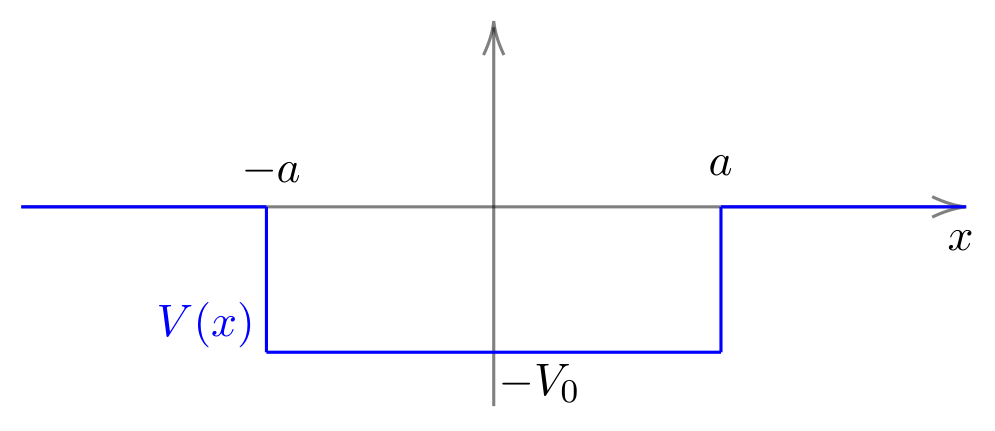
\includegraphics[width=0.60\textwidth]{figures/fig_p40_a.png}
\end{center}
% [图：原书 p.39，原图无题注]

\subsection{匹配条件}

考虑定态薛定谔方程
\[
\left(-\frac{\hbar^2}{2m}\frac{\rd^2}{\rd x^2}+V(x)\right)\psi(x)=E\psi(x).
\]
① 在区域 $\abs{x}>a$ 内，方程变为
\[
-\frac{\hbar^2}{2m}\frac{\rd^2}{\rd x^2}\psi(x)=E\psi,
\]
它有两个线性无关的解
\[
\ee^{\pm\sqrt{-2mE}\,x/\hbar}.
\]
解 $\psi$ 可写成线性组合
\[
\psi=c_1\ee^{\sqrt{-2mE}\,x/\hbar}+c_2\ee^{-\sqrt{-2mE}\,x/\hbar}.
\]

% [原文 p.40]
系数 $c_1,c_2$ 有待确定。解 $\psi$ 在区域 $\abs{x}>a$ 内光滑。

② 在区域 $\abs{x}<a$ 内，方程变为
\[
-\frac{\hbar^2}{2m}\frac{\rd^2}{\rd x^2}\psi=(E+V_0)\,\psi.
\]
同样，$\psi$ 可写成两个无关解的线性组合
\[
\ee^{\pm\sqrt{-2m(E+V_0)}\,x/\hbar}.
\]
$\psi$ 在区域 $\abs{x}<a$ 内也光滑。

由 ①② 可见，$\psi$ 失去光滑性的唯一可能之处是 $x=\pm a$。在 $x=\pm a$ 处应加的自然边界条件为
\begin{equation*}
\psi\ \text{与}\ \psi'\ \text{在}\ x=\pm a\ \text{处连续}.
\tag{$*$}
\end{equation*}
否则 $\psi''$ 在 $x=\pm a$ 处会带上 $\delta$ 函数项，破坏薛定谔方程。我们把这一边界条件 $(*)$ 称为\emph{衔接条件}（matching condition）。

\subsection{束缚态}

先考虑解 $\psi$ 可归一化的情形。这样的能量本征态称为\emph{束缚态}（bound state）。

在区域 $\abs{x}>a$ 内，$\psi(x)$ 是
\[
\ee^{\pm\sqrt{-2mE}\,x/\hbar}
\]
的线性组合。

要使这样的 $\psi$ 可归一化，必须 $E<0$，且
\[
\psi(x)=
\begin{cases}
\alpha\ee^{\sqrt{-2mE}\,x/\hbar}, & x<-a\\
\beta\ee^{-\sqrt{-2mE}\,x/\hbar}, & x>a
\end{cases}
\]
其中 $\alpha,\beta$ 是常数。

另一方面，方程
\[
\left(-\frac{\hbar^2}{2m}\frac{\rd^2}{\rd x^2}+V(x)\right)\psi=E\psi
\]
蕴含
\[
\left\langle\psi\,\Big|\,-\frac{\hbar^2}{2m}\frac{\rd^2}{\rd x^2}\psi\right\rangle
=\langle\psi|(E-V(x))\psi\rangle,
\]
即
\[
\int\rd x\,(E-V(x))\abs{\psi(x)}^2
=\frac{\hbar^2}{2m}\int\rd x\,\abs{\psi'(x)}^2.
\]
要得到非平凡解 $\psi$，必须 $E>\inf_x V(x)=-V_0$。所以束缚态只出现在能量满足
\[
-V_0<E<0
\]
的情形。

% [原文 p.41]
\begin{center}
  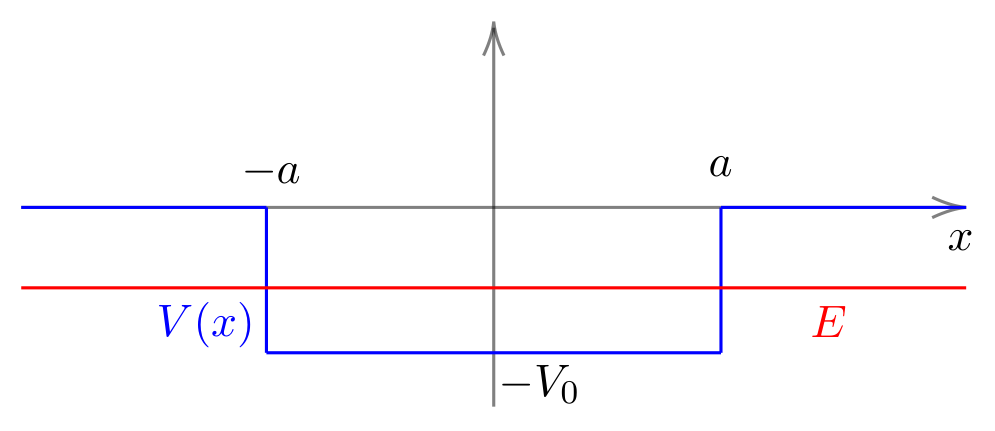
\includegraphics[width=0.62\textwidth]{figures/fig_p42_a.png}
\end{center}
% [图：原书 p.41，原图无题注]

设此成立。则在阱内 $\abs{x}<a$ 处，$\psi$ 是
\[
\cos\left(\frac{\sqrt{2m(E+V_0)}\,x}{\hbar}\right)
\qquad\text{与}\qquad
\sin\left(\frac{\sqrt{2m(E+V_0)}\,x}{\hbar}\right)
\]
的线性组合。

为简化记号，记
\[
\lambda=\frac{\sqrt{-2mE}}{\hbar},
\qquad
\mu=\frac{\sqrt{2m(E+V_0)}}{\hbar}.
\]
还能进一步简化，注意势是偶函数
\[
V(x)=V(-x).
\]
若 $\psi(x)$ 是解，则 $\psi(-x)$ 也是解。因此任一解都可写成偶解与奇解之和
\[
\psi(x)=\frac12\left(\psi(x)+\psi(-x)\right)+\frac12\left(\psi(x)-\psi(-x)\right).
\]
不失一般性，可设 $\psi$ 是偶函数或奇函数。

先设 $\psi$ 为偶函数。则
\[
\psi(x)=
\begin{cases}
\alpha\ee^{-\lambda x}, & x>a\\
\beta\cos\mu x, & \abs{x}<a\\
\alpha\ee^{\lambda x}, & x<-a
\end{cases}
\qquad \alpha,\beta\ \text{是常数}.
\]
现在用衔接条件。由于 $\psi(x)$ 是偶函数，只需考虑 $x=a$ 处。
\[
\begin{cases}
\lim\limits_{x\to a^-}\psi(x)=\lim\limits_{x\to a^+}\psi(x)\\[2mm]
\lim\limits_{x\to a^-}\psi'(x)=\lim\limits_{x\to a^+}\psi'(x)
\end{cases}
\]
由此得到
\[
\begin{cases}
\beta\cos\mu a=\alpha\ee^{-\lambda a}\\[1mm]
-\beta\mu\sin\mu a=-\alpha\lambda\ee^{-\lambda a}
\end{cases}
\]
两式相除，得
\begin{equation*}
\lambda=\mu\tan\mu a.
\tag{$**$}
\end{equation*}
回忆 $\lambda=\sqrt{-2mE}/\hbar$，$\mu=\sqrt{2m(E+V_0)}/\hbar$。上式给出允许的能量。给定满足关系 $(**)$ 的 $E$，可解出 $\psi(x)$，它相差一个归一化因子唯一。于是对应能量 $E$ 的物理态唯一。

% [原文 p.42]
为理解 $(**)$ 的解，重新设
\[
\begin{cases}
u=\mu a=\dfrac{\sqrt{2m(E+V_0)}\,a}{\hbar}\\[3mm]
u_0=\dfrac{\sqrt{2mV_0}\,a}{\hbar}
\end{cases}
\]
我们可以用 $u,u_0$ 表示 $\lambda,\mu$：
\[
\begin{cases}
\mu=\dfrac{u}{a}\\[3mm]
\lambda=\sqrt{\left(\dfrac{u_0}{a}\right)^2-\mu^2}
=\dfrac{\sqrt{u_0^2-u^2}}{a}
\end{cases}
\]
于是方程 $(**)$ 变为
\[
\sqrt{\left(\frac{u_0}{u}\right)^2-1}=\tan u.
\]
其解由曲线 $y=\sqrt{(u_0/u)^2-1}$ 与曲线 $y=\tan u$（$0<u<u_0$）的交点给出。

\begin{center}
  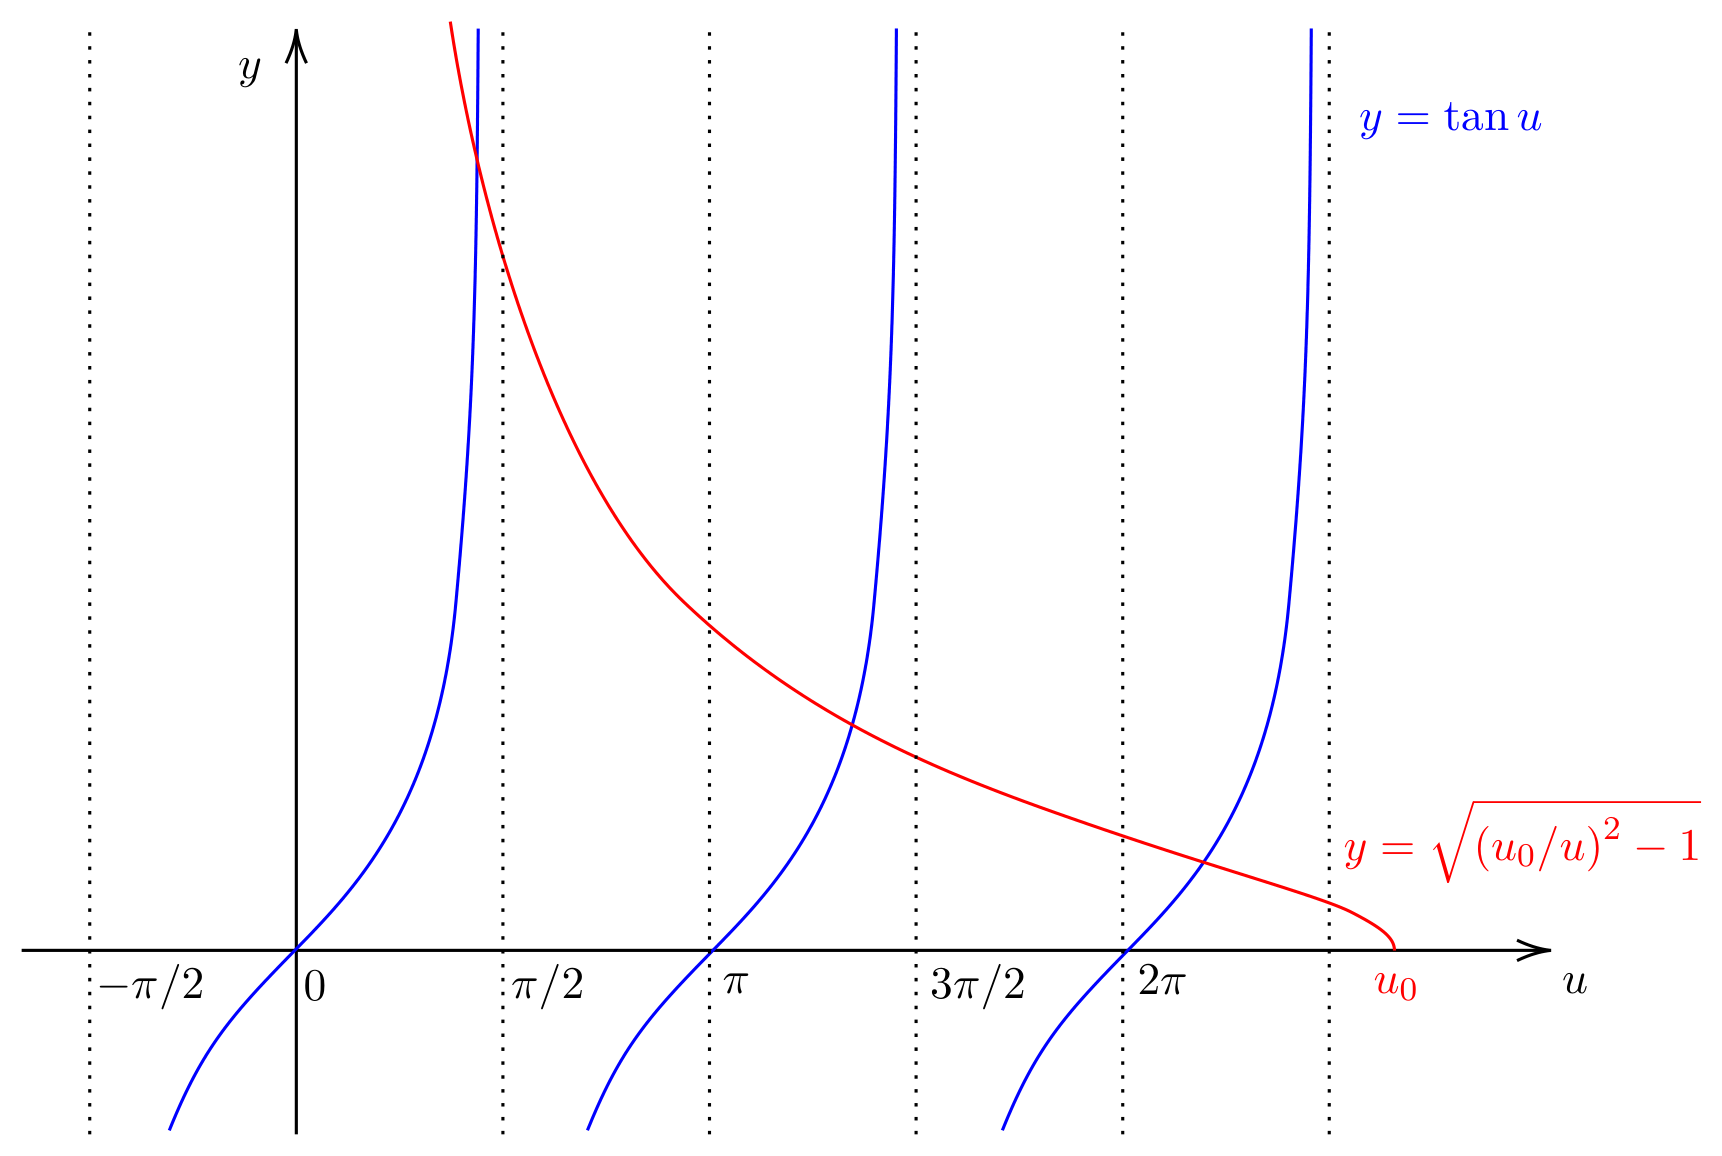
\includegraphics[width=0.75\textwidth]{figures/fig_p43_a.png}
\end{center}
% [图：原书 p.42，原图无题注]

特别地，图表明交点只有有限多个，即允许的能量只有有限多个。交点的个数取决于 $u_0$ 的值。$u_0$ 越大，也就是阱越宽越深，束缚态就越多。但无论如何，至少有一个解，$u_0$ 再小也不例外。

下面简述 $\psi$ 为奇函数的情形。此时
\[
\psi(x)=
\begin{cases}
\alpha\ee^{-\lambda x}, & x>a\\
\beta\sin\mu x, & \abs{x}<a\\
-\alpha\ee^{\lambda x}, & x<-a
\end{cases}
\]

% [原文 p.43]
在 $x=a$ 处的衔接条件给出
\[
\begin{cases}
\beta\sin\mu a=\alpha\ee^{-\lambda a}\\[1mm]
\beta\mu\cos\mu a=-\alpha\lambda\ee^{-\lambda a}
\end{cases}
\]
由此得到 $E$ 所需满足的关系
\[
\mu\cot\mu a=-\lambda.
\]
仍用上面的变量 $u$ 与 $u_0$，这即
\[
\sqrt{\left(\frac{u_0}{u}\right)^2-1}=-\cot u.
\]
在 $0<u<u_0$ 上画出相应的曲线

\begin{center}
  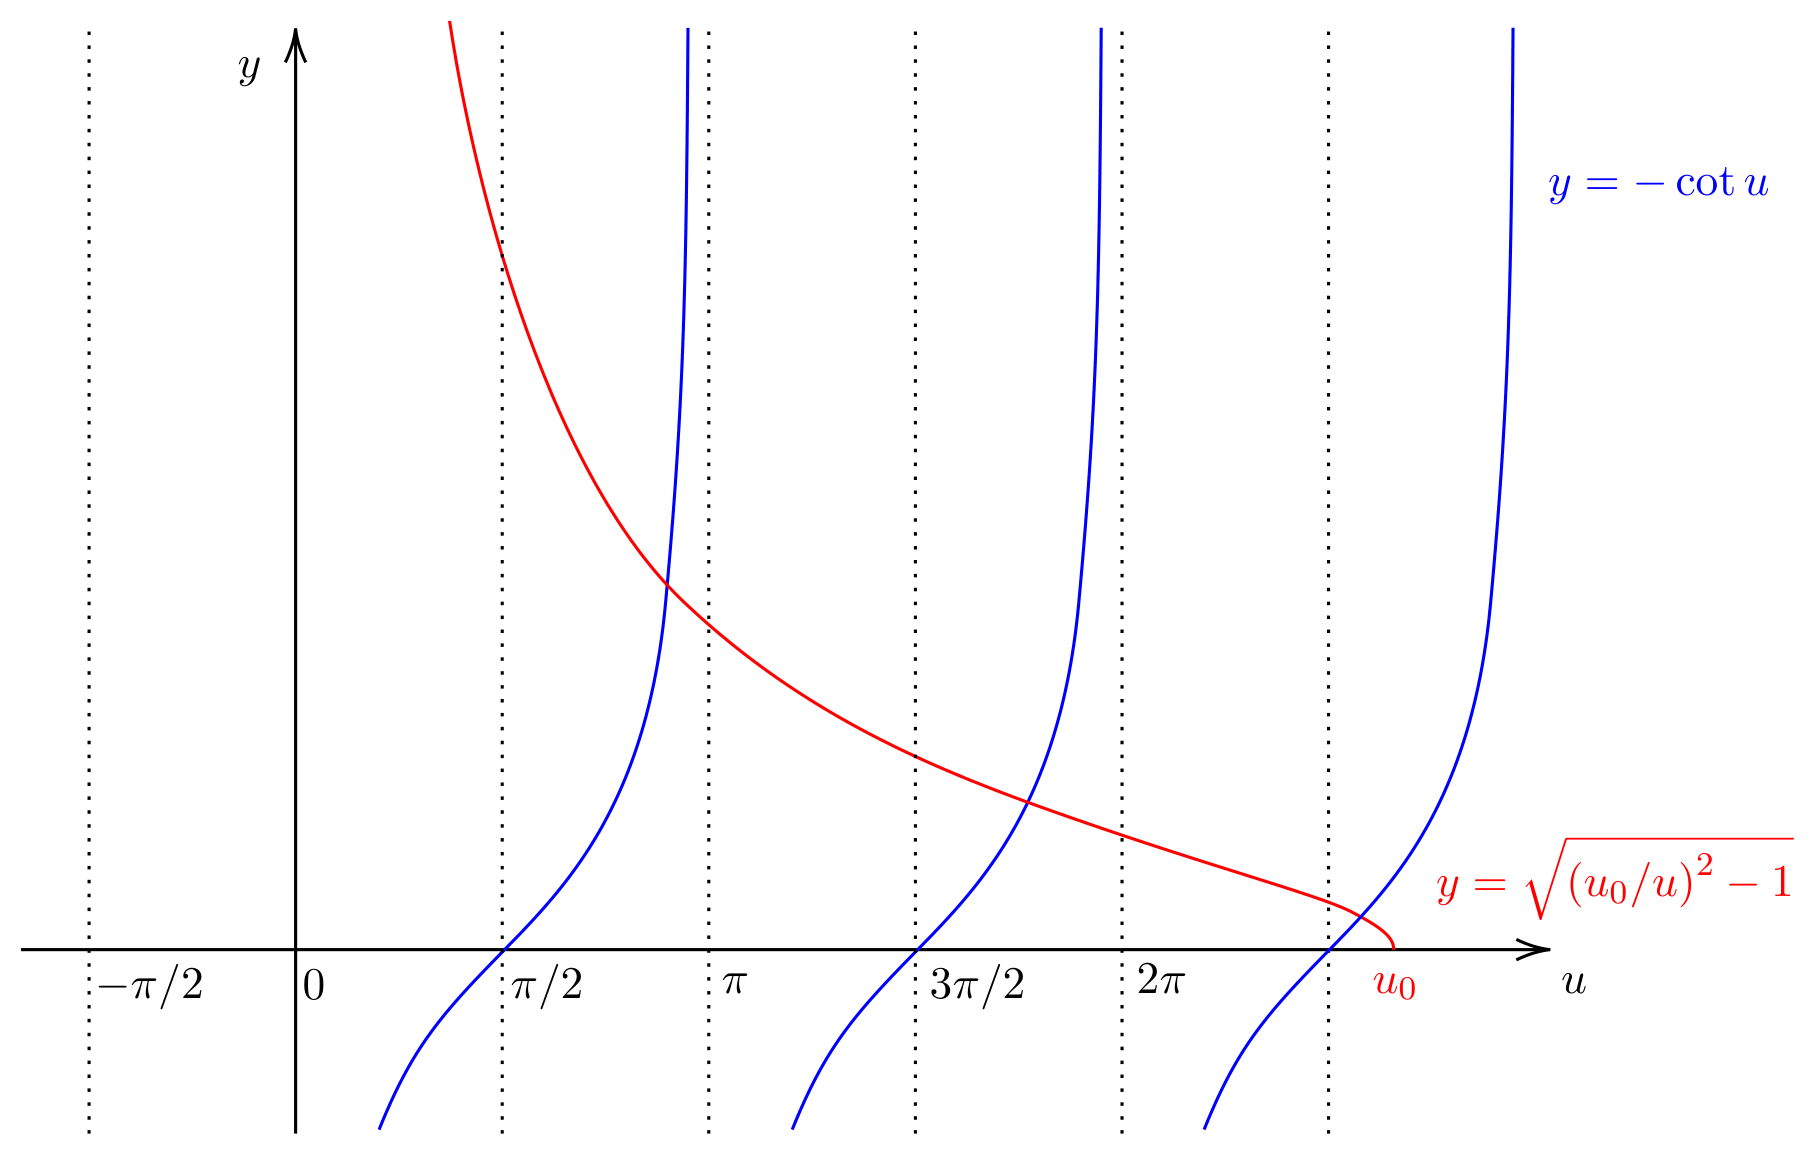
\includegraphics[width=0.75\textwidth]{figures/fig_p44_a.png}
\end{center}
% [图：原书 p.43，原图无题注]

同样，交点只有有限多个。$u_0$ 越大，奇束缚态越多，也就是阱越宽越深。不过，$u_0$ 充分小，例如 $u_0<\pi/2$，就不会有奇束缚态。

总结一下，我们求得有限多个能量
\[
-V_0<E_0<E_1<\cdots<E_N<0,
\]
每个 $E_i$ 恰有一个束缚态 $\psi_i(x)$。$i$ 为偶（奇）时波函数 $\psi_i(x)$ 为偶（奇）函数。基态 $\psi_0$ 是偶函数，且总是存在。

\begin{center}
  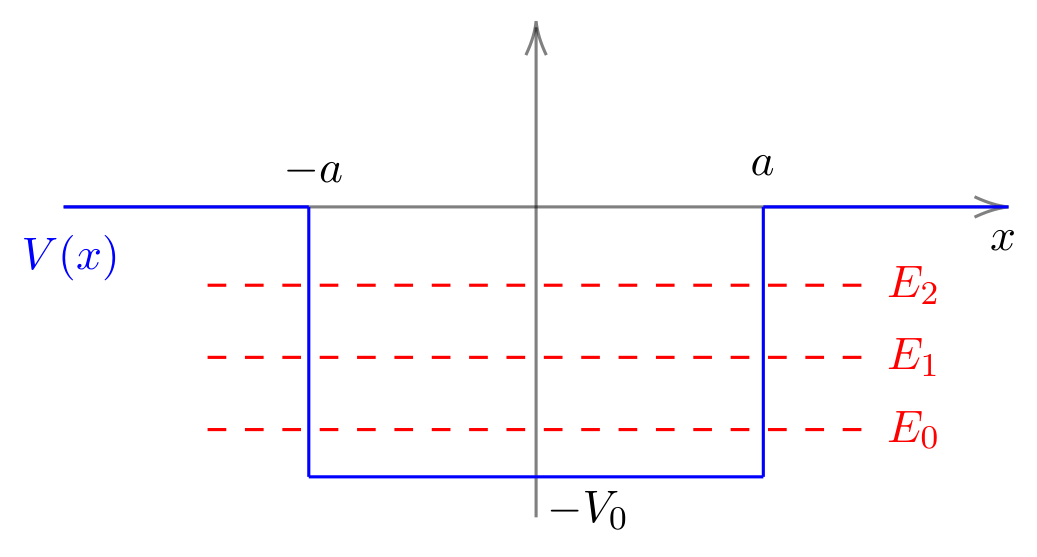
\includegraphics[width=0.62\textwidth]{figures/fig_p44_b.png}
\end{center}
% [图：原书 p.43，原图无题注]

% [原文 p.44]
\begin{center}
  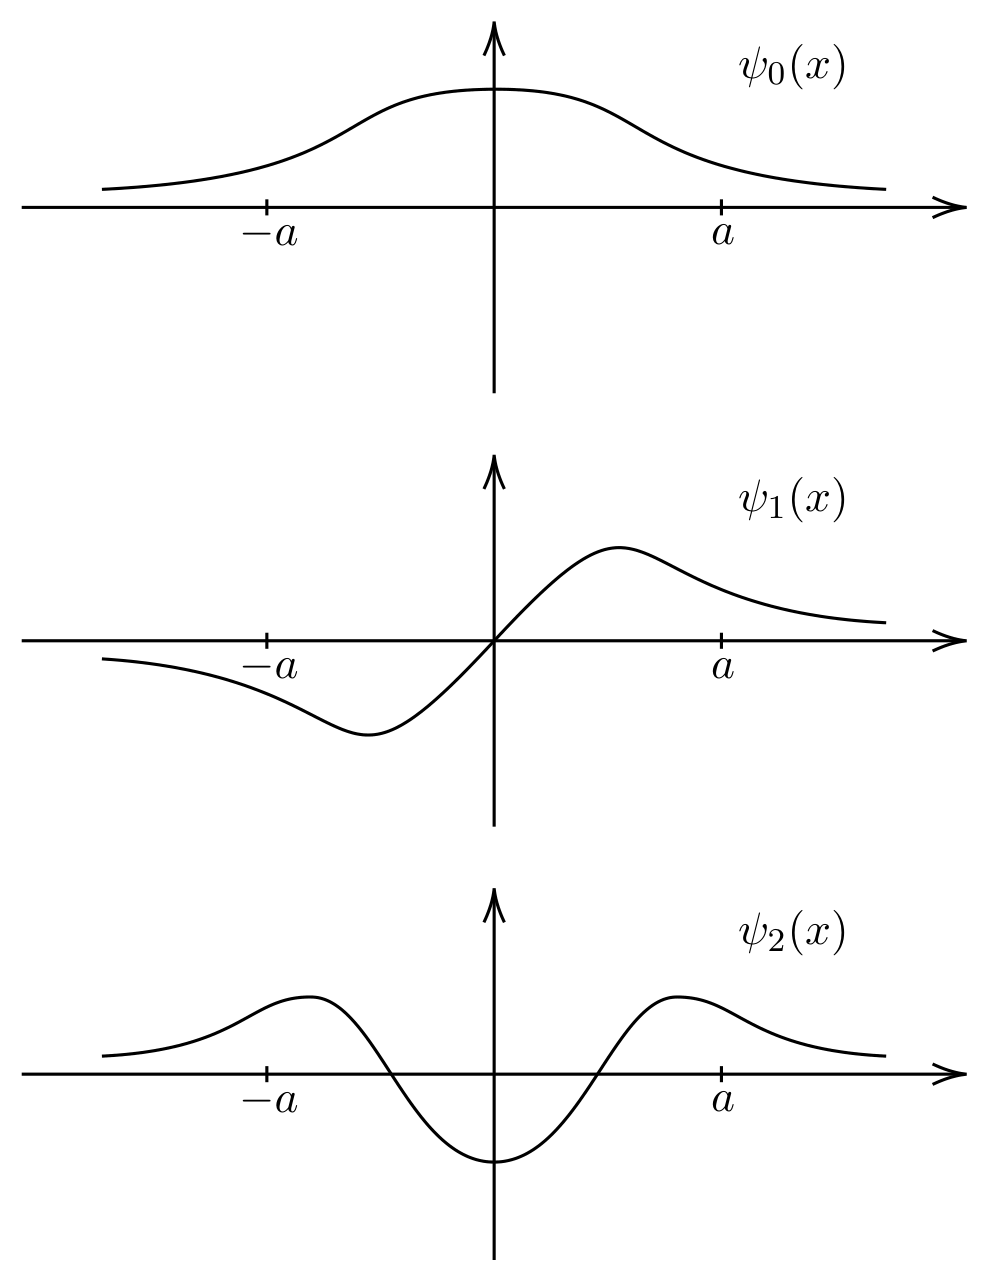
\includegraphics[width=0.52\textwidth]{figures/fig_p45_a.png}
\end{center}
% [图：原书 p.44，原图无题注]

下面简述极限情形 $V_0\to+\infty$。这对应 $u_0\to+\infty$。

\begin{center}
\begin{tabular}{cc}
  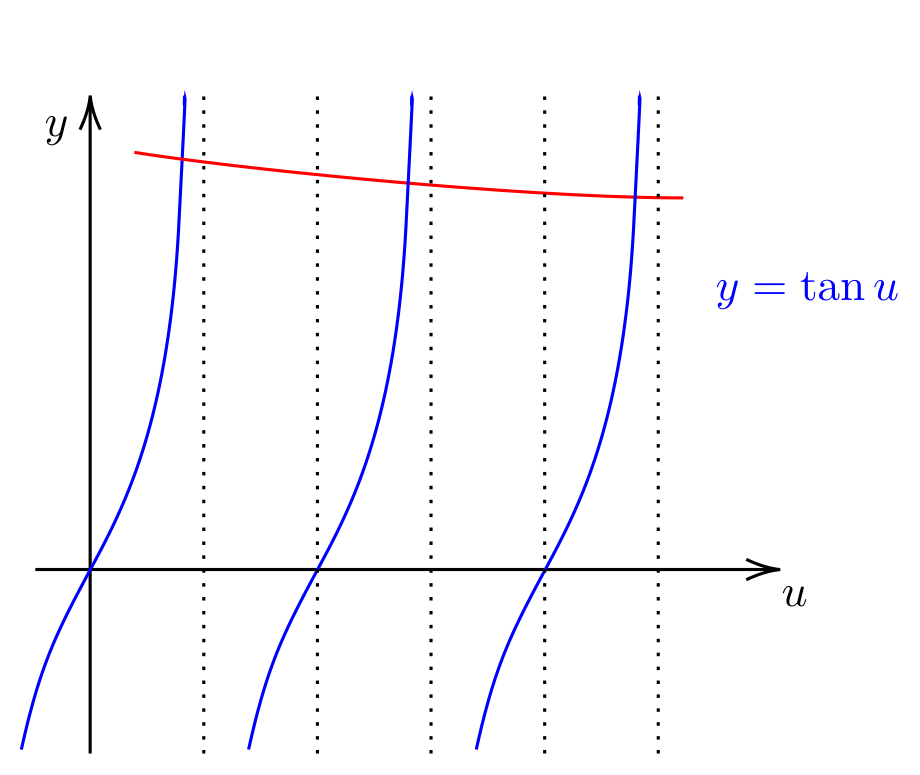
\includegraphics[width=0.42\textwidth]{figures/fig_p45_b.png} &
  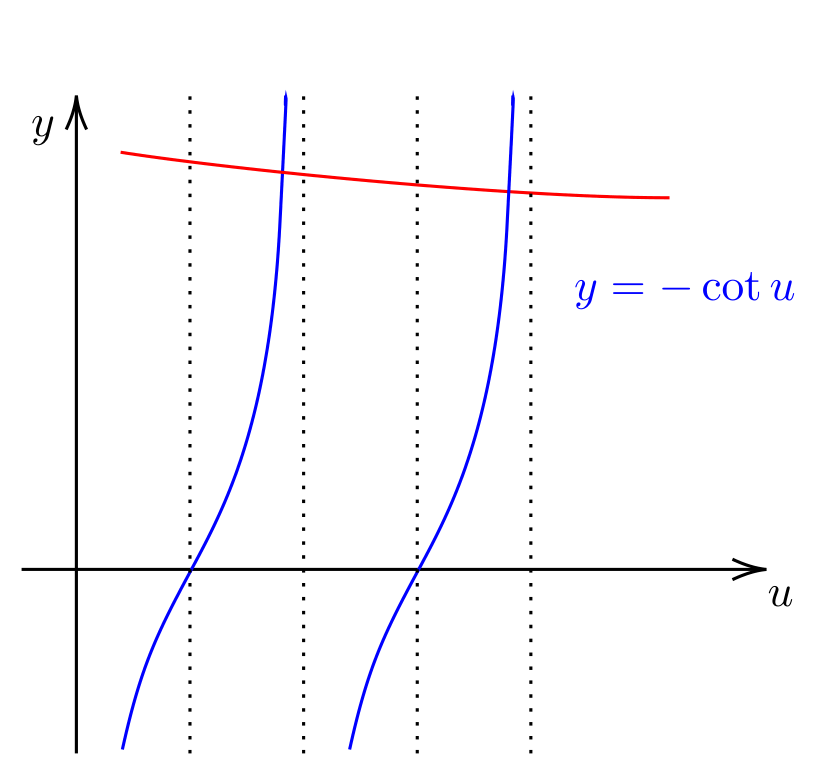
\includegraphics[width=0.42\textwidth]{figures/fig_p45_c.png} \\
  偶情形 & 奇情形
\end{tabular}
\end{center}
% [图：原书 p.44，原图无题注；原图下方英文小标注 even case / odd case，已译为中文]

在这个深阱极限下，交点近似出现在 $u$ 为 $\pi/2$ 的整数倍处。由此可知
\[
\sqrt{2m(E_n+V_0)}\,\frac{a}{\hbar}\simeq\frac{(n+1)\pi}{2}
\quad\Longrightarrow\quad
E_n+V_0\simeq\frac{(n+1)^2\pi^2\hbar^2}{2m(2a)^2},
\qquad n=0,1,2,\cdots
\]
令人惊讶的是，下一节讨论散射问题时，这个公式会再次出现在共振透射里。
% 原文 "Surprisedly" 拼写有误（应为 "Surprisingly"），纯拼写问题，不进正文批注。

% [原文 p.45]
\subsection{散射态}

我们已经看到，方势阱只有有限多个束缚态。束缚态能量对应哈密顿量 $\hat H$ 的离散谱。谐振子中束缚态构成希尔伯特空间的一组基；方势阱的束缚态空间却是有限维的，因而不能张满整个希尔伯特空间。与自由粒子情形一样，$\hat H$ 还会有连续谱。事实上，$x$ 离得远时势为零，粒子在那里就像自由粒子。这提示定态薛定谔方程存在不可归一化的解，它们在远处表现为自由粒子的平面波。稍后就会看到，确实如此。这些解称为\emph{散射态}（scattering states）。名称的由来将在 §1.9 解释。

$E>0$ 时出现散射态。

\begin{center}
  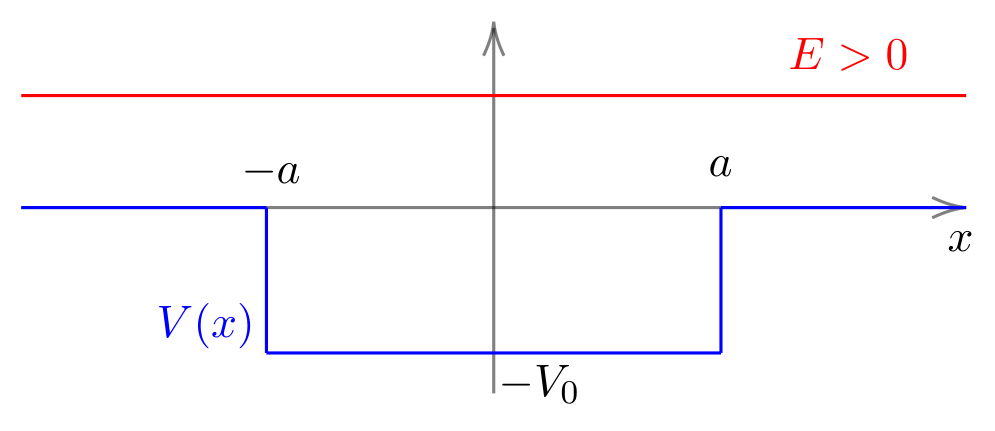
\includegraphics[width=0.62\textwidth]{figures/fig_p46_a.png}
\end{center}
% [图：原书 p.45，原图无题注]

定态薛定谔方程
\[
\left(-\frac{\hbar^2}{2m}\frac{\rd^2}{\rd x^2}+V(x)\right)\psi=E\psi
\]
可以像束缚态那样逐区求解。
\[
\psi(x)=
\begin{cases}
A\ee^{\ii kx}+B\ee^{-\ii kx}, & x<-a\\
C\sin\mu x+D\cos\mu x, & -a<x<a\\
F\ee^{\ii kx}+G\ee^{-\ii kx}, & x>a
\end{cases}
\]
这里 $A,B,C,D,F,G$ 是常数，且
\[
k=\frac{\sqrt{2mE}}{\hbar}>0,
\qquad
\mu=\frac{\sqrt{2m(E+V_0)}}{\hbar}>0.
\]
在 $x=\pm a$ 处，再次施加衔接条件。

由于 $E>0$，当 $x\to\infty$ 时波函数 $\psi(x)$ 振荡而不衰减，因此不可归一化。不过，这类解正是散射过程的构件，§1.9 将讨论这一点。先说明基本想法。设
\[
\psi(x,t)=\psi(x)\ee^{-\ii Et/\hbar}
\]
是含时薛定谔方程的相应解。看区域 $x<-a$，此处
\[
\psi(x,t)=A\ee^{\ii\left(kx-\frac{\hbar k^2}{2m}t\right)}
+B\ee^{-\ii\left(kx+\frac{\hbar k^2}{2m}t\right)}.
\]
第一项 $A\ee^{\ii\left(kx-\frac{\hbar k^2}{2m}t\right)}$ 是以相速度 $\frac{\hbar k}{2m}$ 向右行进的平面波；第二项 $B\ee^{-\ii\left(kx+\frac{\hbar k^2}{2m}t\right)}$ 是以同一相速度向左行进的平面波。

% [原文 p.46]
按上述解释，我们考虑形如
\[
\psi(x)=
\begin{cases}
A\ee^{\ii kx}+B\ee^{-\ii kx}, & x<-a\\
C\sin\mu x+D\cos\mu x, & -a<x<a\\
F\ee^{\ii kx}, & x>a
\end{cases}
\]
的定态解。

\begin{center}
\begin{tikzpicture}[scale=0.9,>=Stealth]
  \draw[thick] (-3.2,0.5) -- (-1,0.5) -- (-1,-0.5) -- (1,-0.5) -- (1,0.5) -- (3.2,0.5);
  \draw[->,decorate,decoration={snake,amplitude=1.1pt,segment length=5pt}]
    (-2.7,1.55) -- (-1.2,1.55);
  \node[above] at (-1.95,1.6) {\small $A$};
  \draw[->,decorate,decoration={snake,amplitude=1.1pt,segment length=5pt}]
    (-1.2,1.05) -- (-2.7,1.05);
  \node[below] at (-1.95,1.0) {\small $B$};
\end{tikzpicture}
\end{center}
% [图：原书 p.46，本图按原文重绘，图内标注已译为中文；原图无题注]

这个波函数表示如下过程：振幅为 $A$ 的波从左侧 $x=-\infty$ 入射，遇到方势阱；随后振幅为 $B$ 的波被反射回左侧，而振幅为 $F$ 的波穿过方势阱，在 $x=+\infty$ 处向右行进。

\begin{center}
\begin{tikzpicture}[scale=0.9,>=Stealth]
  \draw[thick] (-3.2,0.5) -- (-1,0.5) -- (-1,-0.5) -- (1,-0.5) -- (1,0.5) -- (3.2,0.5);
  \draw[->,decorate,decoration={snake,amplitude=1.1pt,segment length=5pt}]
    (-2.7,1.55) -- (-1.2,1.55);
  \node[above] at (-1.95,1.6) {\small $A$};
  \draw[->,decorate,decoration={snake,amplitude=1.1pt,segment length=5pt}]
    (-1.2,1.05) -- (-2.7,1.05);
  \node[below] at (-1.95,1.0) {\small $B$};
  \draw[->,decorate,decoration={snake,amplitude=1.1pt,segment length=5pt}]
    (1.2,1.55) -- (2.7,1.55);
  \node[above] at (1.95,1.6) {\small $F$};
  \node[anchor=west] at (-2.2,-1.05) {\small $A$：入射波振幅};
  \node[anchor=west] at (-2.2,-1.55) {\small $B$：反射波振幅};
  \node[anchor=west] at (-2.2,-2.05) {\small $F$：透射波振幅};
\end{tikzpicture}
\end{center}
% [图：原书 p.46，本图按原文重绘，图内标注已译为中文；原图无题注]

定义
\[
\begin{aligned}
\text{反射系数：}\quad & R=\frac{\abs{B}^2}{\abs{A}^2},\\[2mm]
\text{透射系数：}\quad & T=\frac{\abs{F}^2}{\abs{A}^2}.
\end{aligned}
\]
$R$ 表示反射的概率，$T$ 表示透射的概率。由这一物理含义，应当期望
\[
T+R=1.
\]
一种看法是用概率守恒的局部形式。回忆 §1.5.4 中的概率流
\[
j(x)=\frac{\hbar}{m}\Imag\left(\overline{\psi}\frac{\rd}{\rd x}\psi\right).
\]
把它代入上面的 $\psi$，得
\[
j(x)=
\begin{cases}
\dfrac{\hbar k}{m}\left(\abs{A}^2-\abs{B}^2\right), & x<-a\\[3mm]
\dfrac{\hbar k}{m}\abs{F}^2, & x>a
\end{cases}
\]

% [原文 p.47]
对定态解，概率密度 $\rho$ 不随时间变化。守恒方程
\[
\frac{\pa\rho}{\pa t}+\frac{\pa}{\pa x}j(x)=0
\]
表明 $j(x)$ 必与 $x$ 无关：概率不能在空间任何区域堆积。由此可知
\[
\abs{A}^2=\abs{B}^2+\abs{F}^2
\quad\Longrightarrow\quad
T+R=1.
\]

下面用衔接条件解出 $\psi(x)$。
\[
x=-a:\quad
\begin{cases}
A\ee^{-\ii ka}+B\ee^{\ii ka}=-C\sin\mu a+D\cos\mu a\\[1mm]
\ii k\left(A\ee^{-\ii ka}-B\ee^{\ii ka}\right)=\mu\left(C\cos\mu a+D\sin\mu a\right)
\end{cases}
\]
\[
x=a:\quad
\begin{cases}
C\sin\mu a+D\cos\mu a=F\ee^{\ii ka}\\[1mm]
\mu\left(C\cos\mu a-D\sin\mu a\right)=\ii kF\ee^{\ii ka}
\end{cases}
\]
这四个方程（在整体归一化之下）唯一确定五个常数 $A,B,C,D,F$。经过一番冗长的计算，得到
\[
\begin{cases}
\dfrac{F}{A}=\dfrac{\ee^{-2\ii ka}}
{\cos 2\mu a-\ii\dfrac{\sin 2\mu a}{2k\mu}\left(k^2+\mu^2\right)}\\[6mm]
\dfrac{B}{F}=\ii\dfrac{\sin 2\mu a}{2k\mu}\left(\mu^2-k^2\right)
\end{cases}
\]
于是可算出反射系数 $R$、透射系数 $T$，并验证前面断言的 $T+R=1$。显式地，透射概率为
\[
T=\frac{\abs{F}^2}{\abs{A}^2}
=\frac{1}{1+\dfrac{V_0^2}{4E(E+V_0)}\sin^2\left(\dfrac{2a}{\hbar}\sqrt{2m(E+V_0)}\right)}.
\]
$T$ 作为 $E$ 的函数，图像如下

\begin{center}
  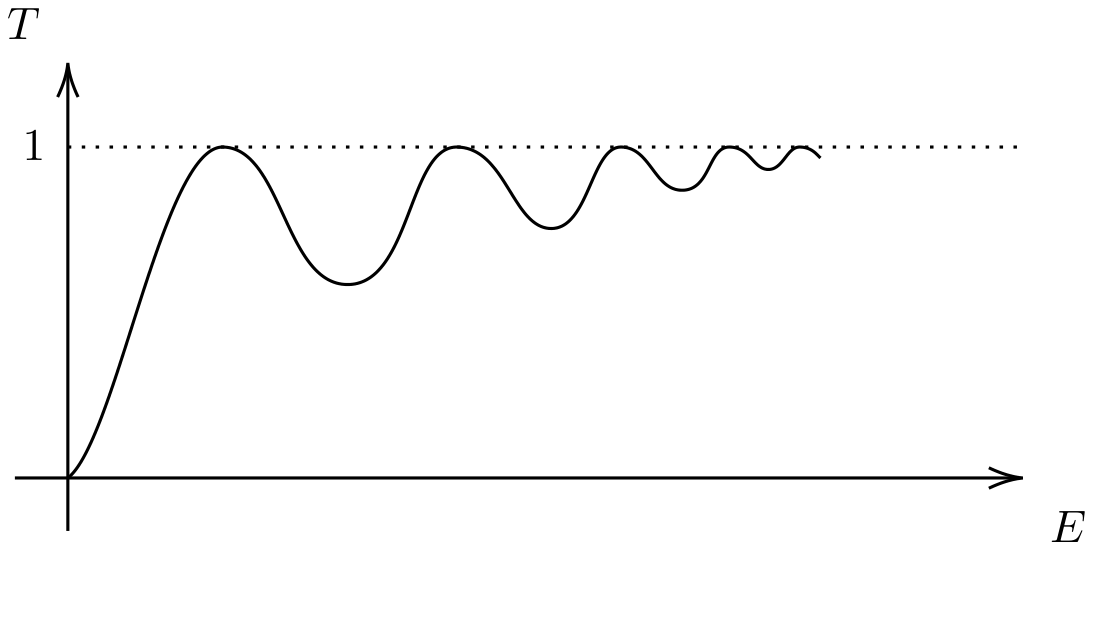
\includegraphics[width=0.62\textwidth]{figures/fig_p48_a.png}
\end{center}
% [图：原书 p.47，原图无题注]

注意，存在某些 $E$ 使 $T=1$。此时完全透射，没有任何波被反射：势阱变得透明！由 $T$ 的上述公式，完全透射发生在
\[
E_n+V_0=\frac{(n+1)^2\pi^2\hbar^2}{2m(2a)^2},
\qquad n\in\Z\ \text{且}\ E_n>0.
\]

\takeaway{有限深方势阱兼有离散谱与连续谱：$-V_0<E<0$ 时有有限多个束缚态，能量由衔接条件定出，基态为偶函数；$E>0$ 时为不可归一化的散射态，透射系数在共振能量处等于一。}

% [本块止于原书 p.47，下接 ch01c]

